\PassOptionsToPackage{dvipsnames}{xcolor}

\documentclass[12pt]{beamer}
\usetheme{default}
\usecolortheme{crane}

\usepackage[utf8x]{inputenc}
\usepackage[T1]{fontenc}
\usepackage[slovak]{babel}
\usepackage{ucs} % unicode

\usepackage{amsmath}
\usepackage{amsmath, amssymb}
\usepackage{hyperref, url}
\usepackage{graphicx}
\usepackage{array}
\usepackage{alltt}

%\setbeamersize{text margin left=1pt,text margin right=1pt}
\setbeamertemplate{footline}[frame number]
\beamertemplatenavigationsymbolsempty

% https://www.overleaf.com/learn/latex/Using_colours_in_LaTeX
\def\blue#1{\textcolor{Cerulean}{#1}}
\def\green#1{\textcolor{LimeGreen}{#1}}

% database-related stuff
\DeclareMathOperator{\join}{\bowtie}
\DeclareMathOperator{\antijoin}{\rhd}

\DeclareMathOperator{\lubi}{lubi}
\DeclareMathOperator{\capuje}{capuje}
\DeclareMathOperator{\navstivil}{navstivil}
\DeclareMathOperator{\vypil}{vypil}
\DeclareMathOperator{\answer}{answer}

\title{Navrhovanie databáz}
\author{Ján Mazák}
\institute{FMFI UK Bratislava}
\date{}


\begin{document}

\frame{\titlepage}

\begin{frame}[fragile]{Návrh databázových schém}
\alert{Databázová schéma}: čo sú atribúty a aký majú dátový typ, aké relácie máme, vzťahy medzi nimi.
\bigskip

Pri návrhu databázovej schémy (voľne databázy) sa najmä snažíme vyhnúť známym nedostatkom.
Neraz ide o kompromis medzi blízkosťou k ideálnemu návrhu a výkonom v praxi.
\bigskip

Relačný model, jazyk SQL a bežné DBMS poskytujú dostatok prostriedkov na zabezpečenie integrity dát.
\end{frame}

\begin{frame}[fragile]{Entitno-relačný model}
Pri návrhu vychádzame zo zjednodušeného modelu sveta --- \emph{dátový model}.
Tieto modely sa bežne kreslia v podobe \alert{entitno-relačných diagramov} (ERM/ERD).
\begin{itemize}
\item entitám v tomto modeli zodpovedajú tabuľky,\\ ich atribútom stĺpce
\item vzťahy 1:N reprezentujeme atribútmi
\item vzťahy M:N zvyčajne reprezentujeme tabuľkami
(atribút, ktorého dátovým typom je pole, je takmer vždy v rozpore s dobrou praxou)
\end{itemize}
\end{frame}

\begin{frame}[fragile]{Entitno-relačný model}
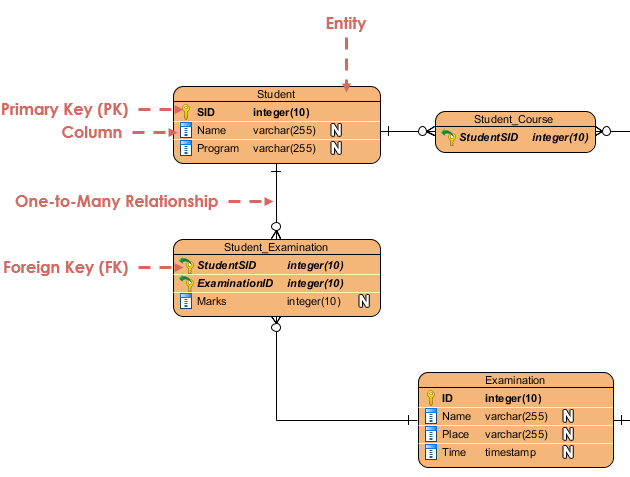
\includegraphics[scale=.5]{erd.png}
\end{frame}


\begin{frame}[fragile]{Nedostatky v návrhu}
\begin{itemize}
\item zlý či neaktuálny dátový model\\ (bežné pri digitalizácii verejnej správy)
\item nejasnosti v tom, aké dáta sú potrebné a či je možné ich získať
\item schéma, ktorú je ťažké upraviť pri zmene dátového modelu
      (napr. kvôli nadmernému využitiu custom riešení miesto štandardizovaných; voľte jednoduchosť)
\item zlé pomenovania (nejasné, málo špecifické, nekonzistentné, opakovanie názvu pre rôzne veci)
\item nadmerné použitie indexov (netreba ich \uv{pre každý prípad} pre každý atribút)
\item chýbajúca dokumentácia, najmä zdôvodnenia netriviálnych rozhodnutí
\end{itemize}
\end{frame}

\begin{frame}[fragile]{Nedostatky v návrhu --- redundancia}
\begin{tabular}{|c|c|c|}
\hline
\emph{Zamestnanec} & \emph{Pracovisko} & \emph{Adresa pracoviska} \\\hline
Adam & SAV & Patrónka \\\hline
Adam & KAGDM & Mlynská dolina \\\hline
Cyril & KAGDM & Mlynská dolina \\\hline
\end{tabular}
\bigskip

\alert{Redundancy}: Informácia o adrese pracoviska je v tabuľke viacnásobne.
\end{frame}

\begin{frame}[fragile]{Nedostatky v návrhu --- anomálie pri updatovaní}
\begin{tabular}{|c|c|c|}
\hline
\emph{Zamestnanec} & \emph{Pracovisko} & \emph{Adresa pracoviska} \\\hline
Adam & SAV & Patrónka \\\hline
Adam & KAGDM & Mlynská dolina \alert{$\rightarrow$ Staré grunty}\\\hline
Cyril & KAGDM & Mlynská dolina \\\hline
\end{tabular}
\bigskip

\alert{UPDATE anomaly}: keď upravíme adresu pracoviska v jednom zázname, bude to v rozpore s ostatnými záznamami.
\end{frame}

\begin{frame}[fragile]{Nedostatky v návrhu --- anomálie pri mazaní}
\begin{tabular}{|c|c|c|}
\hline
\emph{Zamestnanec} & \emph{Pracovisko} & \emph{Adresa pracoviska} \\\hline
Adam & SAV & Patrónka \\\hline
Adam & KAGDM & Mlynská dolina \\\hline
Cyril & KAGDM & Mlynská dolina \\\hline
\end{tabular}
\bigskip

\alert{DELETE anomaly}: keď zmažeme všetkých zamestnancov pracoviska, stratíme informáciu o jeho adrese.
\end{frame}

\begin{frame}[fragile]{Nedostatky v návrhu --- anomálie pri vkladaní}
\begin{tabular}{|c|c|c|}
\hline
\emph{Zamestnanec} & \emph{Pracovisko} & \emph{Adresa pracoviska} \\\hline
Adam & SAV & Patrónka \\\hline
Adam & KAGDM & Mlynská dolina \\\hline
Cyril & KAGDM & Mlynská dolina \\\hline
\end{tabular}
\bigskip

\alert{INSERT anomaly}: nemožno zmysluplne pridať adresu pracoviska bez pridania zamestnancov (resp. NULL).
\end{frame}

\begin{frame}[fragile]{Nedostatky v návrhu --- ako sa im vyhnúť?}
Riešenie: dekompozícia relácií.

\bigskip
\begin{tabular}{|c|c|c|}
\hline
\emph{Zamestnanec} & \emph{Pracovisko} \\\hline
Adam & SAV \\\hline
Adam & KAGDM \\\hline
Cyril & KAGDM \\\hline
\end{tabular}
\begin{tabular}{|c|c|c|}
\hline
\emph{Pracovisko} & \emph{Adresa prac.} \\\hline
SAV & Patrónka \\\hline
KAGDM & Mlynská d. \\\hline
\end{tabular}
\bigskip

\begin{itemize}
\item žiadna redundancia
\item žiadne anomálie (INSERT, UPDATE, DELETE)
\end{itemize}

\bigskip
Naplnenie relácií v dekompozícii získame projekciou z pôvodnej relácie.
Pôvodné dáta získame pomocou operácie JOIN.
\end{frame}

\let\fz\rightarrow

\begin{frame}[fragile]{Funkčné závislosti}
Ako vieme, podľa ktorých atribútov robiť dekompozíciu a kedy už je dostatočná?
Matematický model: funkčné závislosti.
\bigskip

Uvažujme reláciu $R$ a dve množiny atribútov $X$, $Y$.\\
\alert{Funkčná závislosť} $X\fz Y$ platí práve vtedy,\\
keď \green{pre každé naplnenie relácie $R$} platí:\\
\blue{ak sa dva záznamy zhodujú na všetkých atribútoch z $X$, zhodujú sa aj na všetkých atribútoch z $Y$}.
\bigskip

Príklad: R = (Meno, RodnéČíslo, ČísloPasu); FZ:\\
$\{\hbox{RodnéČíslo}\}\fz \{\hbox{Meno}\}$\\
$\{\hbox{RodnéČíslo, Meno}\}\fz \{\hbox{ČísloPasu, Meno}\}$

{\scriptsize ČísloPasu môže byť NULL, preto sa nehodí na identifikáciu záznamu.
FZ to nepokazí, lebo NULL hodnota nie je rovná žiadnej inej, ani NULL, a môžeme použiť UNIQUE.}
\end{frame}

\begin{frame}[fragile]{Funkčné závislosti a kľúče}
FZ nemožno identifikovať z naplnenia databázy (pri inom by nemuseli platiť), musia byť preto súčasťou návrhu.
Pomocou FZ vieme vyjadriť napr. pojem kľúča.
\bigskip

Množina atribútov $X$ je v nejakej relácii s atribútmi $R$ \alert{nadkľúč}, ak platí $X\fz R$.
Nadkľúč minimálny vzhľadom na inklúziu sa nazýva \alert{kľúč}.
(V angličtine sa pre dvojicu pojmov nadkľúč/kľúč používa superkey/key alebo key/candidate key.)
\bigskip

Aké kľúče má relácia (Meno, RodnéČíslo, ČísloPasu)?
\end{frame}

\begin{frame}[fragile]{Primary keys}
V relácii (Meno, RodnéČíslo, ČísloPasu) sú atribúty RodnéČíslo a ČísloPasu kľúčmi.
Pre externé nástroje je výhodné, keď možno záznamy identikovať úplne jednoznačne,
preto si zo všetkých kľúčov chceme vybrať primárny.
\begin{itemize}
\item PostgreSQL: \alert{PRIMARY KEY} = NOT NULL UNIQUE.
\item SQLite: PRIMARY KEY je unique, ale \emph{nie} NOT NULL.\\
      {\scriptsize \url{https://www.sqlitetutorial.net/sqlite-primary-key/}}
\end{itemize}

\bigskip
Primárny kľúč môže zahŕňať viac atribútov:
\begin{alltt}
CREATE TABLE ta (
  a1 integer, a2 integer,
  \alert{PRIMARY KEY (a1, a2)}
);
\end{alltt}
\end{frame}

\begin{frame}[fragile]{Primary keys}
Pre niektoré tabuľky nemáme žiadnych prirodzených kandidátov na primárny kľúč
(napr. ak tabuľka len zachytáva vzťah M:N). Vtedy môžeme pridať ako primárny kľúč
\alert{umelý identifikátor}, ktorý jednoznačne identifikuje záznam.

\begin{itemize}
\item PostgreSQL: SERIAL.
\item SQLite: atribút definovaný ako INTEGER PRIMARY KEY je automaticky aliasom pre ROWID
(stĺpec s automaticky inkrementovanými hodnotami).
\end{itemize}

Umelé id možno využiť, aj keď máme iné kľúče, napr. ak sa chceme vyhnúť kompozitným kľúčom
či pridlhým hodnotám kľúčových atribútov (index nad celými číslami zaberá menej miesta
a je rýchlejší než nad dlhými reťazcami).
\end{frame}

\begin{frame}[fragile]{Funkčné závislosti}
Reprezentácia funkčných závislostí v SQL: pomocou UNIQUE.
\bigskip

Pre závislosť $AB\fz C$ spravíme tabuľku
\begin{alltt}
      CREATE TABLE t (
            A <data_type_of_A>,
            B <data_type_of_B>,
            C <data_type_of_C>,
            \alert{UNIQUE(A, B)}
      );
\end{alltt}
Keďže sa do nej nedajú vložiť záznamy $(a_1, b_1, c_1)$ a $(a_1, b_1, c_2)$, platí aj požadovaná funkčná závislosť.
\end{frame}

\begin{frame}[fragile]{Funkčné závislosti}
Aké funkčné závislosti musia platiť pre nasledujúcu reláciu? (Hľadáme závislosti vynútené SQL kódom.)
\begin{alltt}
    CREATE TABLE customers (
        id        integer PRIMARY KEY,     ---- I
        address   text NOT NULL,           ---- A
        name      text NOT NULL,           ---- N
        email     text NOT NULL UNIQUE,    ---- E
        phone     text NOT NULL UNIQUE,    ---- P
        UNIQUE(name, address)
    );
\end{alltt}
\pause
\begin{itemize}
\item PRIMARY KEY: $I\fz ANEP$
\item UNIQUE: $E\fz I$, $P\fz I$, $AN\fz I$
\item Z významu stĺpcov to vyzerá tak, že iné FZ (okrem tých, čo vyplývajú z uvedených) už medzi týmito atribútmi nie sú (a nechceme ich v SQL vynucovať).
\end{itemize}
\end{frame}

\begin{frame}[fragile]{Funkčné závislosti}
Funkčné závislosti treba vnímať so všetkými ich dôsledkami. Predpokladajme, že platí
$$
A\fz C,\quad B\fz D,\quad CD\fz E.
$$
Potom aj
\begin{eqnarray*}
AB\fz D\\
A\fz A\\
AB\fz E\\
\dots
\end{eqnarray*}
\end{frame}

\begin{frame}[fragile]{Funkčné závislosti}
Pravidlá pre odvodzovanie --- Armstrongove axiómy.
\begin{enumerate}
\item Ak $X\fz Y$, tak $XZ\fz YZ$.
\item Ak $Y \subseteq X$, tak $X\fz Y$.
\item Ak $X\fz Y$ a $Y\fz Z$, tak $X\fz Z$.
\end{enumerate}
Ich platnosť vyplýva priamo z definície FZ.
\bigskip

Odvodiť sa dajú ďalšie pravidlá, napr.
$A_1A_2\dots A_n\fz B_1B_2\dots B_n\ \leftrightarrow\ \forall i\ A_1A_2\dots A_n\fz B_i$.
\bigskip

Množinu všetkých FZ, ktoré možno odvodiť z danej množiny FZ $M$, nazývame \alert{uzáver množiny FZ} $M$.\\
(Jeho veľkosť môže byť exponenciálna vzhľadom na veľkosť $M$, čo spôsobuje algoritmické problémy.)
\end{frame}

\begin{frame}[fragile]{Funkčné závislosti}
\alert{Uzáver množiny atribútov} $\{A_1,A_2\dots,A_n\}$ vzhľadom na nejakú množinu FZ $M$:
maximálna množina atribútov $B$ taká, že platí $A_1A_2\dots A_n\fz B$.

\bigskip
Uzáver možno vypočítať v polynomiálnom čase tak, že začneme pôvodnou množinou atribútov,
a v každom kroku prejdeme všetky FZ z $M$ a pre každú z nich pridáme do uzáveru pravú stranu,
ak sa tam už nachádza ľavá strana. Keď sme nič nepridali počas celého prechodu $M$, končíme.

\bigskip
Uzáver možno využiť na overenie, či je daná množina atribútov kľúč (ako?),
alebo na výpočet všetkých FZ platných v danej relácii
(vyskúšame všetky možné podmnožiny atribútov ako ľavé strany
a na pravú stranu pripíšeme uzáver ľavej strany).
\end{frame}


\begin{frame}[fragile]{Dekompozícia relácií}
V princípe každú databázu možno vnímať ako jedinú reláciu (predstavte si join všetkých tabuliek).
Preto dekompozícia relácie na menšie je pri návrhu kľúčová, aj keď ju explicitne nevnímame.
\bigskip

Pri dekompozícii \alert{nechceme polámať funkčné závislosti}.
\bigskip

Príklad: relácia $order\_items(Order, Product, Amount)$ so závislosťou
$$\{Order, Product\}\fz \{Amount\}.$$
Ak ju akokoľvek dekomponujeme, stratíme informáciu o tom, že $\{Order, Product\}$ je kľúč.
Pri kontrole integrity budeme musieť pri každej zmene niektorej z čiastkových relácií spočítať join a overiť,
či nedošlo k porušeniu FZ.
\end{frame}

\begin{frame}[fragile]{Dekompozícia relácií --- bezstratovosť}
Z dekomponovanej relácie musíme vedieť získať pôvodné záznamy.
Inak povedané, ak spravíme join, dostaneme práve pôvodné záznamy a \green{nič navyše} ---
nestratili sme žiadnu informáciu, čiže ide o \alert{bezstratovú dekompozíciu} (\alert{lossless decomposition}).

\bigskip
Otestovať, či je dekompozícia bezstratová, možno polynomiálnym algoritmom
(link: \href{https://en.wikipedia.org/wiki/Chase\_(algorithm)}{chase algorithm}).

\bigskip
Jednoduchšie riešenie pre 2 relácie:
požadujeme, aby množina spoločných atribútov bola v aspoň jednej z nich nadkľúčom.
\end{frame}

\begin{frame}[fragile]{Dekompozícia relácií --- bezstratovosť}
\blue{$r(Zamestnanec, Pracovisko, AdresaPracoviska)$}\\
dekomponujeme na\\
\green{$r_1(Zamestnanec, Pracovisko)$},\\
\green{$r_2(Pracovisko, AdresaPracoviska)$}.\\
Je táto dekompozícia bezstratová?
\pause

\bigskip
Označme $Z = Zamestnanec$, $P = Pracovisko$, $A = AdresaPracoviska$.\\[2mm]
V $r$ platia FZ $Z\fz P$, $P\fz A$. Preto $P$ ($= r_1\cap r_2$) je kľúč v $r_2$ a do (natural) joinu $r_1\bowtie r_2$
sa nemôže dostať záznam, ktorý v $r$ nebol, pretože tento join ku každému riadku $r_1$ len doplní hodnotu $A$ z $r_2$.
\end{frame}

\begin{frame}[fragile]{Dekompozícia relácií}
Požiadavky na dekompozíciu:
\begin{itemize}
\item \green{Je bezstratová.} (Nutné.)
\item \blue{Neláme funkčné závislosti.} (Z tohto sa dá trocha zľaviť,
            ale je oveľa lepšie FZ zachovať, umožňuje to kontrolu integrity štandardnými prostriedkami.)
\item \alert{Odstraňuje čo najviac redundancie a anomálií.}
\end{itemize}
Redundancia sa odstraňuje \alert{normalizáciou} --- cieleným dekomponovaním.
Mieru normalizácie popisujú \alert{normálne formy}.
\end{frame}

\begin{frame}[fragile]{Normálne formy}
\begin{itemize}
\item[\alert{1NF}] Nemáme duplikáty ani kompozitné atribúty\\ (hodnotou atribútu nie je relácia).
\item[\alert{3NF}] Odstraňuje väčšinu redundancie a problémov s anomáliami. Vždy existuje a ľahko sa hľadá.
\item[\alert{BCNF}] Čosi ako 3.5NF, ideál. Relácia v BCNF neobsahuje žiadnu redundanciu vzhľadom na FZ, ani nedochádza k spomínaným anomáliám.
\end{itemize}
Normálne formy vytvárajú hierarchiu (ak je niečo vo vyššej, je aj v nižšej).
Existujú aj vyššie normálne formy (napr. 4NF), tie sa venujú odstraňovaniu tzv. multivalued dependencies.
V praxi sú zväčša irelevantné.
\end{frame}

\begin{frame}[fragile]{BCNF}
Relácia $r$ je v BCNF, ak \green{ľavá strana každej netriviálnej FZ je nadkľúč} $r$.

\bigskip
Problémy:
\begin{itemize}
\item Pre niektoré relácie neexistuje\\ (napr. $r(ABC)$, kde FZ sú $AB\fz C$, $C\fz A$).
\item Pre danú reláciu je NP-úplné rozhodnúť, či je v BCNF.
\end{itemize}

\bigskip
Ak relácia $R$ nie je v BCNF kvôli FZ $X\fz Y$, dekomponujeme ju do $XY$ a $R-Y$.
(Zachováva bezstratovosť.)

(V literatúre možno nájsť iné, hoci ekvivalentné, definície jednotlivých normálnych foriem.
BCNF nemá pekné číslo: zámerom bolo už v 3NF odstrániť všetku redundanciu,
ale vyšlo to až na druhý pokus.)
\end{frame}

\begin{frame}[fragile]{3NF}
Relácia $r$ je v 3NF, ak \green{ľavá strana každej netriviálnej FZ je nadkľúč} $r$
alebo každý atribút na pravej strane je súčasťou nejakého kľúča.

\bigskip
Vlastnosti:
\begin{itemize}
\item Pre danú reláciu je NP-úplné rozhodnúť, či je v 3NF.
\item Dekompozícia do 3NF vždy existuje.
\item Existuje polynomiálny algoritmus, ktorý aspoň jednu 3NF nájde (cez minimálne pokrytie).
Nájdená dekompozícia je bezstratová a zachováva FZ.
\end{itemize}

\bigskip
Schéma vytvorená na základe dobrého entitno-relačného modelu je zväčša už v 3NF.
\end{frame}

\begin{frame}[fragile]{Normalizácia}
Normalizujme reláciu $R$:\\[2mm]
\begin{tabular}{|c|c|c|}
\hline
\emph{Zamestnanec $Z$} & \emph{Pracovisko $P$} & \emph{Adresa pracoviska $A$} \\\hline
Adam & KAGDM & Mlynská dolina \\\hline
Cyril & KAGDM & Mlynská dolina \\\hline
\end{tabular}
\pause

\bigskip
FZ: $Z\fz P$, $P\fz A$. Jediný kľúč je $Z$.

\bigskip
FZ \alert{$P\fz A$} porušuje BCNF, lebo ľavá strana nie je nadkľúč.\\
Aj $3NF$, lebo atribút $A$ na pravej strane nie je súčasťou žiadneho kľúča.

\bigskip
Preto dekomponujeme: do \green{$PA$} a $R - A = \green{ZP}$.\\
Tie sú binárne, preto v BCNF. FZ ostali zachované.
\end{frame}

\begin{frame}{Užitočná redundancia}
Ak máme veľa dát, možno nechceme opakovane rátať agregačné funkcie, povedzme súčet.
Jeho hodnotu $H$ možno vypočítať dopredu, napr. tak, že záznamy dostávajú timestamp,
podľa ktorého je spravený BTREE index, a v rámci dotazu počítame
len $H$ k nejakému timestampu plus záznamy, ktoré pribudli.

\bigskip
V takom prípade treba strážiť konzistenciu dát: pri zmene hodnôt originálnych záznamov
(napr. zmazanie najstarších) aktualizovať $H$ a naopak nedovoliť zmenu $H$ bez úpravy originálnych záznamov.

\bigskip
Mechanizmus: \alert{trigger} --- funkcia uložená v databáze, ktorá sa spustí zakaždým,
keď nastane definovaná udalosť, napr. pred pridaním či po pridaní riadka.
\end{frame}

\begin{frame}[fragile]{Normalizácia}
Prehnaná normalizácia vedie k binárnym reláciám\\
(tie sú vždy v BCNF).

\bigskip
Príklad: binárne relácie\\
(Id, Meno), (Id, Priezvisko), (Id, RodneCislo)\\
miesto\\
(Id, Meno, Priezvisko, RodneCislo).

\bigskip
Zaužívané pravidlá je pri normalizácii občas výhodné porušiť,
treba však mať jasno, že prečo, a uviesť to v dokumentácii.
Kompromis medzi zachovaním FZ a znížením redundancie nemá
jediné správne objektívne riešenie, treba sa riadiť skúsenosťou.
\end{frame}


\begin{frame}[fragile]{Foreign keys}
Atribút obsiahnutý v niekoľkých reláciách:
\begin{itemize}
\item V matematickom relačnom modeli vždy \uv{ten istý}.
\item V SQL rovnako pomenované stĺpce v rôznych tabuľkách nemajú medzi sebou žiaden vzťah.
\end{itemize}
\alert{Foreign keys} (cudzie kľúče) --- mechanizmus na zabezpečenie súladu hodnôt toho istého atribútu v rôznych tabuľkách (referenčná integrita).
\end{frame}

\begin{frame}[fragile]{Foreign keys}
\begin{alltt}
CREATE TABLE ta (
  a1 integer \alert{REFERENCES tb},
  a2 integer,
  a3 integer,
  \alert{FOREIGN KEY (a2, a3) REFERENCES tc (c1, c2)}
);
\end{alltt}
Cudzie kľúče možno pomenovať (ľahšie sa tak identifikuje dôvod zamietnutia operácie):
{\scriptsize
\begin{alltt}
  CONSTRAINT fk_name1 FOREIGN KEY a1 REFERENCES tb (b1)
  CONSTRAINT fk_name2 FOREIGN KEY (a2, a3) REFERENCES tc (c1, c2)
\end{alltt}
}
\end{frame}

\begin{frame}[fragile]{Foreign keys}
\hbox{}{\small
\begin{alltt}
CREATE TABLE products (
  product_no integer PRIMARY KEY,
  price numeric
);
CREATE TABLE orders (
  order_id integer PRIMARY KEY
);
CREATE TABLE order_items (
  order_id integer \alert{REFERENCES orders} \blue{ON DELETE CASCADE},
  product_no integer \alert{REFERENCES products}
      \blue{ON DELETE RESTRICT ON UPDATE CASCADE},
  quantity integer,
  PRIMARY KEY (product_no, order_id)
);
\end{alltt}
}
\end{frame}

\begin{frame}[fragile]{Foreign keys}
Možnosti pre \blue{ON DELETE}
\begin{itemize}
\item \alert{CASCADE} -- zmaže riadok, ktorý sa odkazoval na mazaný riadok
\item \alert{RESTRICT} -- nezmaže nič, operácia DELETE skončí s chybou
\item SET NULL -- nastaví odkaz na NULL\\ (zlyhá pre NOT NULL stĺpce)
\item SET DEFAULT -- nastaví hodnotu odkazu na defaultnú
(zlyhá, ak takto vznikne nekorektný odkaz)
\item NO ACTION -- toto je default, DELETE skončí s chybou
\end{itemize}
\end{frame}

\begin{frame}[fragile]{Foreign keys}
Možnosti pre \blue{ON UPDATE}
\begin{itemize}
\item \alert{CASCADE} -- zmení odkazujúcu hodnotu na novú hodnotu odkazovanej
(zachová väzbu medzi riadkami)
\item RESTRICT -- zabráni zmene v odkazovanej tabuľke, UPDATE zlyhá
\item SET NULL -- nastaví odkaz na NULL (väzba zanikne)
\item SET DEFAULT -- nastaví hodnotu odkazu na defaultnú
(zlyhá, ak takto vznikne nekorektný odkaz)
\item NO ACTION -- toto je default, väzba sa pokazí
\end{itemize}
\end{frame}

\begin{frame}[fragile]{Foreign keys}
Kedy sa vyhodnocuje platnosť odkazu?
\begin{itemize}
\item \alert{DEFERRED} -- až pri commite transakcie
\item \alert{IMMEDIATE} -- okamžite po vykonaní operácie
\end{itemize}
\pause
Možnosti pri definícii cudzieho kľúča:
\begin{itemize}
\item \green{NOT DEFERRABLE} -- vždy okamžité vyhodnocovanie
\item \green{DEFERRABLE INITIALLY IMMEDIATE} -- v rámci tx možno zvoliť, kedy vyhodnocovať, default je ihneď
\item \green{DEFERRABLE INITIALLY DEFERRED} -- v rámci tx možno zvoliť, kedy vyhodnocovať, default je commit
\end{itemize}
\end{frame}


\begin{frame}{Literatúra}
\begin{itemize}
\item {\scriptsize\href{https://www.lucidchart.com/pages/er-diagrams}{entity-relationship diagrams}}
\item {\scriptsize\href{https://en.wikipedia.org/wiki/Database_normalization}{normal forms}}
\item {\scriptsize\href{https://mariadb.com/kb/en/database-normalization-overview/}{normalization example 1}}
\item {\scriptsize\href{https://www.databasestar.com/database-normalization/}{normalization example 2}}
\item {\scriptsize\url{https://www.postgresql.org/docs/current/ddl-constraints.html}}
\item {\scriptsize\url{https://www.postgresql.org/docs/current/sql-set-constraints.html}}
\item {\scriptsize\href{https://www.postgresqltutorial.com/postgresql-triggers/creating-first-trigger-postgresql/}{trigger v PostgreSQL}}
\item {\scriptsize\href{https://www.sqlitetutorial.net/sqlite-trigger/}{trigger v SQLite}}
\item {\scriptsize\url{https://www.db-book.com/slides-dir/PDF-dir/ch6.pdf}}
\item {\scriptsize\url{https://www.db-book.com/slides-dir/PDF-dir/ch7.pdf}}
\item {\scriptsize\url{https://cs186berkeley.net/notes/note13/}}
\end{itemize}
\end{frame}


\begin{frame}{Literatúra}
Online normalization tools (limited functionality)
\begin{itemize}
\item {\scriptsize\url{https://www.ict.griffith.edu.au/normalization_tools/normalization/index.html}}
\item {\scriptsize\url{https://arjo129.github.io/functionalDependencyCalculator/}}
\item {\scriptsize\url{http://raymondcho.net/RelationalDatabaseTools/RelationalDatabaseTools.html}}
\item {\scriptsize\url{https://uisacad5.uis.edu/cgi-bin/mcrem2/database_design_tool.cgi}}
\end{itemize}
\end{frame}

\begin{frame}[fragile]{Úloha}
Máme databázu kníh; predpokladáme, že každú napísal jediný autor. Atribúty:\\[3mm]
\begin{minipage}{.4\pdfpagewidth}
\begin{itemize}
\item ISBN
\item Názov
\item Autor
\item NárodnosťAutora
\item Formát
\item Cena
\end{itemize}
\end{minipage}
\begin{minipage}{.4\pdfpagewidth}
\begin{itemize}
\item Témy (zoznam tém)
\item PočetStrán
\item Vydavateľstvo
\item KontaktVydavateľstvo
\item Žáner
\item DefiníciaŽánru
\end{itemize}
\end{minipage}

\bigskip
Identifikujte funkčné závislosti a navrhnite vhodnú databázovú schému v BCNF alebo aspoň v 3NF.
Overte bezstratovosť dekompozície.
\end{frame}

\end{document}
